\documentclass[11pt, a4paper]{article}
%\usepackage{proj1}
\usepackage{natbib}
\usepackage{fancyhdr}  
\usepackage{subcaption}
\usepackage{caption}
\usepackage{graphicx}
\usepackage{numprint}
\usepackage{multirow}
\linespread{1.25} 
\setlength{\parindent}{0cm}
\graphicspath{{Images/}}
\usepackage{hyperref}
\usepackage{amsmath}
\usepackage{amsfonts}
\usepackage{amssymb}
\usepackage{amsthm}
\usepackage{mathtools}
\usepackage{commath}
\usepackage{bbm}

%\usepackage[sc,osf]{mathpazo}
\usepackage{subcaption}
\usepackage[a4paper, top=1in, left=1.0in, right=1.0in, bottom=1in, includehead, includefoot]{geometry} %Usually have top as 1in

\usepackage{listings}
\usepackage{color} %red, green, blue, yellow, cyan, magenta, black, white
\definecolor{mygreen}{RGB}{28,172,0} % color values Red, Green, Blue
\definecolor{mylilas}{RGB}{170,55,241}


\hypersetup{colorlinks,linkcolor={black},citecolor={blue},urlcolor={black}}
\usepackage{color}
\urlstyle{same}


\theoremstyle{definition}
\newtheorem{definition}{Definition}[section]

\newcommand{\adja}{q_a}
\newcommand{\adjb}{q_b}
\newcommand{\adjaB}{q_{a,\partial \Omega}}
\newcommand{\adjbB}{q_{b,\partial \Omega}}
\newcommand{\adjB}{q_{\partial \Omega}}
\newcommand{\Adja}{\mathbf{p}}
\newcommand{\Adjb}{q}
\newcommand{\adj}{q}
\newcommand{\Adjc}{{q}_{\partial \Omega}}
\newcommand{\ra}{\rho_a}
\newcommand{\rb}{\rho_b}
\newcommand{\w}{\mathbf{w}}
\newcommand{\f}{\mathbf{f}}
\newcommand{\ve}{\mathbf{v}}
\newcommand{\n}{\mathbf{n}}
\newcommand{\h}{\mathbf{h}}
\newcommand{\K}{\mathbf{K}}
\newcommand{\hr}{\widehat \rho}

%	\begin{figure}[h]
%		\centering
%		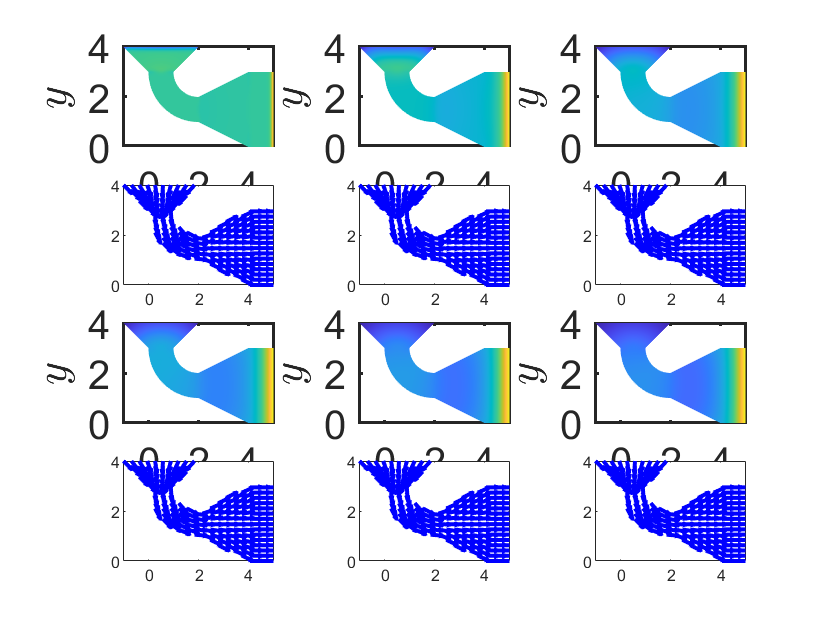
\includegraphics[scale=0.35]{F1.png}
%		\caption{Forward $\rho$ for $a = 0.01$} 
%		\label{F1}
%	\end{figure}

\begin{document}
	
	\section{Multishape OCP}
	(Note: MultiShapeFancyChannel3)
	Last week, there was an issue with the multishape OCP for small $\beta$ in particular. I have found an alternative initial condition for the problem to work. Last week the initial condition was a Gaussian located in the first shape only. This causes the algorithm to converge to $wErr = 0.00$ in only a few iterations, while $J_{FW} < J_{Opt}$. I suspect this is happening because there is not enough mass in the system. When I ran the OCP on the last two shapes without changing the initial condition (by accident) the same mistake occurred, while it didn't occur when I ran it on the first shape. 
	I now changed the initial condition to $\rho_0 = 0.5$. This works well with $\beta = 10^{-3}$ and $J_{FW} = 0.1218$, while $J_{Opt} = 0.0034$. The result can be seen in Figure \ref{F1}.
	\begin{figure}[h]
		\centering
		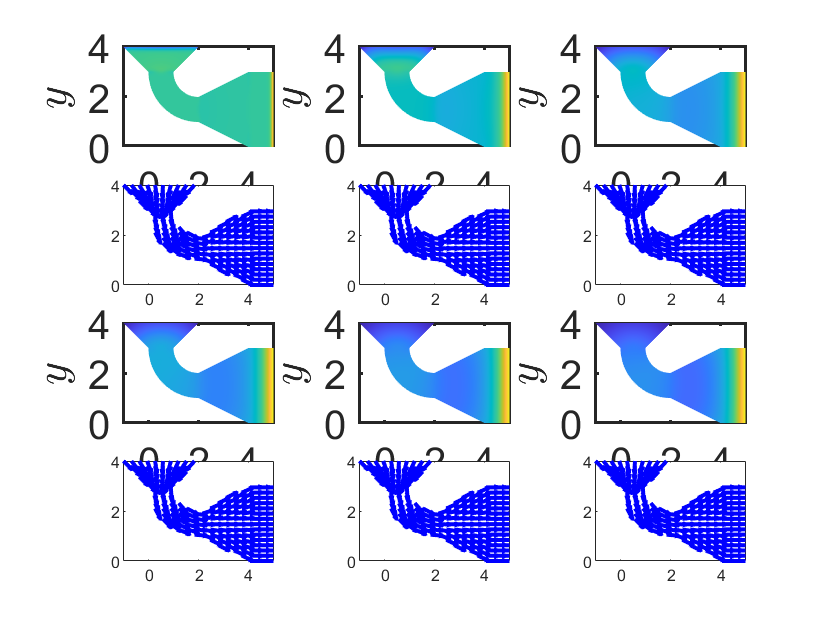
\includegraphics[scale=0.35]{F1.png}
		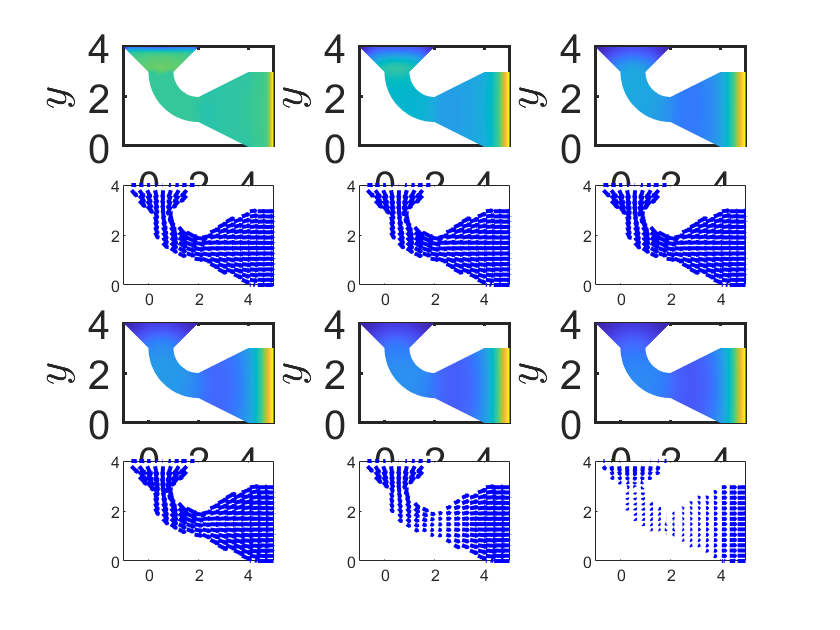
\includegraphics[scale=0.35]{F2.png}
		\caption{$\hr$ and optimal $\rho$ with corresponding $\w$.} 
		\label{F1}
	\end{figure}


	
\section{Periodic Boundary Conditions}
We consider the advection diffusion equation with periodic boundary conditions and a corresponding OCP:
\begin{align*}
	&\min \frac{1}{2}|| \rho - \hr||^2 + \frac{\beta}{2}||\w||^2\\
	&\text{subject to:}\\
	&\frac{\partial \rho}{\partial t} = \frac{\partial^2 \rho}{\partial x^2} - \frac{\partial \rho \w}{\partial x}\\
	& \rho(a) = \rho(b)\\
	& \frac{\partial \rho(a)}{\partial x} - \rho(a) \w(a) = \frac{\partial \rho(b)}{\partial x}  - \rho(b) \w(b)
\end{align*}
The relevant part of the Lagrangian is then:
\begin{align*}
	\mathcal{L} &= ... -\int_0^T \int_\Omega \left(\frac{\partial \rho}{\partial t} - \frac{\partial^2 \rho}{\partial x^2} + \frac{\partial \rho \w}{\partial x}\right)q dr dt \\
	&- \int_0^T \left(-\rho(b)q_1 + \rho(a)q_1 - \frac{\partial \rho(b)}{\partial x}q_2 + \rho(b)\w(b)q_2 + \frac{\partial \rho(a)}{\partial x}q_2 - \rho(a)\w(a)q_2\right) dt.
\end{align*}
Taking partial derivatives, the relevant part of the Lagrangian is:
\begin{align*}
	\mathcal{L} = ... - \int_0^T \left[q \frac{\partial \rho}{\partial x} - \rho\frac{\partial q}{\partial x} - \rho \w q\right]_a^b -
	\left(-\rho(b)q_1 + \rho(a)q_1 - \frac{\partial \rho(b)}{\partial x}q_2 + \rho(b)\w(b)q_2 + \frac{\partial \rho(a)}{\partial x}q_2 - \rho(a)\w(a)q_2\right)dt.
\end{align*}
Taking the derivative with respect to $\rho$ gives:
\begin{align*}
	\mathcal{L}_\rho h &= ... - \int_0^T \left[q \frac{\partial h}{\partial x} - h\frac{\partial q}{\partial x} - h \w q\right]_a^b \\
	&-
	\left(-h(b)q_1 + h(a)q_1 - \frac{\partial h(b)}{\partial x}q_2 + h(b)\w(b)q_2 + \frac{\partial h(a)}{\partial x}q_2 - h(a)\w(a)q_2\right)dt
\end{align*}
Writing all terms explicitly:
\begin{align*}
	\mathcal{L}_\rho h &= ... + \int_0^T \bigg(- q(b) \frac{\partial h(b)}{\partial x} + h(b)\frac{\partial q(b)}{\partial x} + h(b) \w(b) q(b) + q(a) \frac{\partial h (a)}{\partial x} - h(a)\frac{\partial q(a)}{\partial x} - h(a) \w(a) q(a)  \\
	&h(b)q_1 - h(a)q_1 + \frac{\partial h(b)}{\partial x}q_2 - h(b)\w(b)q_2 - \frac{\partial h(a)}{\partial x}q_2 + h(a)\w(a)q_2 \bigg)dt
\end{align*}
Then considering the terms that satisfy $\frac{\partial h}{\partial x} \neq 0$ at $a$ and $b$ separately we get:
\begin{align*}
	&\int_0^T -q(b) \frac{\partial h(b)}{\partial x} + \frac{\partial h(b)}{\partial x} q_2 dt= 0\\
	& \int_0^T q(a) \frac{\partial h (a)}{\partial x} - \frac{\partial h(a)}{\partial x}q_2 dt =0
\end{align*}
	And therefore we find $q(b) = q_2$ and $q(a) = q_2$ and so: 
	\begin{align*}
		q(a) = q(b).
	\end{align*}
Then considering the terms where $h \neq 0$, again separately for $a$ and $b$ we get:
\begin{align*}
	&\int_0^T  h(b)\frac{\partial q(b)}{\partial x} + h(b) \w(b) q(b) + h(b)q_1 - h(b)\w(b)q_2 dt = 0\\
	&\int_0^T - h(a)\frac{\partial q(a)}{\partial x} - h(a) \w(a) q(a) - h(a)q_1 + h(a)\w(a)q_2 dt = 0
\end{align*}
	And using that $q(b) = q_2$ and $q(a) = q_2$ we get:
	\begin{align*}
		\frac{\partial q(b)}{\partial x} + \w(b) q(b) + q_1 - \w(b)q(b)  = 0\\
		- \frac{\partial q(a)}{\partial x} - \w(a) q(a) - q_1 + \w(a)q(a)  = 0
	\end{align*}
	and so:
	\begin{align*}
		\frac{\partial q(b)}{\partial x}  = \frac{\partial q(a)}{\partial x}. 
	\end{align*}
	Therefore, the two boundary conditions for the adjoint equation are:
	\begin{align*}
		q(a) = q(b) \quad \frac{\partial q(b)}{\partial x}  = \frac{\partial q(a)}{\partial x},
	\end{align*}
	as expected.
	
	
	
	
\end{document}